\chapter{Prototype Implementation}
\label{Chapter4}
\lhead{Chapter 4. \emph{Prototype Implementation}}

In this chapter, we implement a prototype based on PTAM \citep{Reference12}. The prototype integrates the five methods in section \ref{VisualizationMethods}. A use case of this system is in section \ref{AUseCase}.

\section{System Architecture}

The mobile device used in the prototype is a SONY VAIO VGN-UX90PS (see appendix \ref{AppendixA}). We base our program on the PTAM reference implementation source code \citep{Reference16} to get the position and orientation of the VAIO. However, this implementation cannot run on the VAIO because it requires a dual core CPU computer to be able to run smoothly. As a result, we connect a MacBook Pro (appendix \ref{AppendixB}) to the VAIO and the PTAM part of the program will run on the MacBook. The architecture is in figure \ref{VAIOMacBookPro}.

The VAIO and the MacBook are connected by a 11 Mbps wireless network. For the sake of quick setup time, the VAIO and the MacBook are connected directly using ad hoc mode, which means that an additional wireless hub is not needed.

The MacBook may run at 54 Mbps, but the VAIO's built-in wireless network card can only run at 11 Mbps. The 11 Mbps is sufficient for the current prototype. For faster network speed, we can attach a 54 Mbps auxiliary wireless network card for the VAIO. We can also use LAN cable for even faster 100 Mbps speed, but the VAIO will be wired to another bulky device, which is not desirable because the mobility of the VAIO is totally lost.

\section{Server-side PTAM}

We modify the original PTAM source code so that the ``video source'' is remotely located on the VAIO, not on the MacBook. We learn a little from Erlang language \citep{Reference17} of how to write concurrent, high-performance systems. Right after the TCP (Transmission Control Protocol) connection between the VAIO and the MackBook is established:

\begin{itemize}
	\item The VAIO continuously feeds frames captured from its camera to the MacBook.
	\item The MacBook continuously feeds position and orientation of the camera of the VAIO to the VAIO.
\end{itemize}

As the above explanation suggests, we use ``push'' instead of ``pull'', one side actively sends data to the other side without having to wait for the request for the data from the other side. In other words we use the mailbox design pattern instead of the RPC (Remote Procedure Call) design pattern, which is slower and requires synchronizing the call and the result (figure \ref{fig:MailboxRPC}).

\begin{figure}[htbp]
	\centering
	\includegraphics{./Figures/mailbox_rpc.png}
	\rule{35em}{0.5pt}
	\caption[Mailbox vs. RPC]{Mailbox (above) vs. RPC (below)}
	\label{fig:MailboxRPC}
\end{figure}

Because PTAM only need grayscale frames, instead of sending all the three RGB color channels of the frames, the VAIO only need to send the brightness Y = 0.3*R + 0.59*G + 0.11*B. To increase the frame rate sent to the MacBook, we further improve the data transmission by the following optimizations:

\begin{itemize}
	\item Send G color channel instead of Y, because G affects Y the most as in the above common equation. This does not affect PTAM. This optimization enormously improves the frame rate because when we send Y, if the image size is 320x240, we must apply the above equation 76800 times for each frame!
	\item Losslessly compress G color channel using the standard library ``zlib''. The compression rate is about 50\%.
\end{itemize}

\begin{table}[tb]
	\begin{center}
		\begin{tabular}{|c|l|l|}
			\hline
			Sent color data & FPS \\
			\hline
			Y               &     \\
			G               &     \\
			compressed G    &     \\
			\hline
		\end{tabular}
		\caption{Frame rate improves when applying frame transmission optimizations}
	\end{center}
\end{table}

The prototype uses frame size of 320x240. This gives smooth frame rate with be above system architecture and optimizations. Bigger frame size allows PTAM to find more feature points, but the following drawbacks pop up:

\begin{itemize}
	\item Data for each frame gets bigger. This increases data transmission time for each frame.
	\item The MacBook must process more data. This decreases the result frame rate.
\end{itemize}

When increasing from 320x240 to 640x480, the frame rate drop about 4 times, and the prototype no longer works smoothly as required in \ref{VisualizationRequirements}. 

\section{PTAM's Map Initializing Problem}

PTAM continuously build and maintain a map of feature points taken from the frames.

\section{Pre-registered Data}

The system does not use a server or any real surveillance camera. In place of those, 3D model of the building of the College of International Studies and the gymnasium (Figure [cite]), together with the hard coded geometry information about the virtual surveillance cameras are used.

\section{History of this prototype}

The prototype described in the above sections is not the only decision choice we have made throughout this research. Previously, we have made others as described below.

\subsection{Hardware -- Prototype with SONY VAIO VGN-UX90PS, Garmin GPSmap 60CSx, and InterSense InertiaCube3}

We have implemented a prototype with the architecture in figure \ref{fig:VAIOGPSGyro}. The GPS device specifications is in appendix \ref{AppendixD}. The GSP and gyrocompass devices provide position and orientation information of the mobile device. Together with the prebuilt CG information, we can overlay CG objects to visualize viewing fields of surveillance cameras. The update rate of the gyrocompass is 180Hz, which is high thus the orientation information is quite good. However, the GPS device error is about 10m, which affects badly the accuracy of the visualization. To improve the GPS device error, model-based tracking method as described in \citep{Reference13} method may be used.

\begin{figure}[htbp]
	\centering
	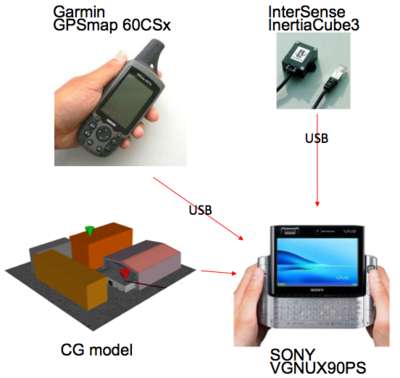
\includegraphics{./Primitives/vaio_gps_gyro.png}
	\rule{35em}{0.5pt}
	\caption[Prototype with SONY VAIO VGN-UX90PS, Garmin GPSmap 60CSx, and InterSense InertiaCube3]{Prototype with SONY VAIO VGN-UX90PS, Garmin GPSmap 60CSx, and InterSense InertiaCube3}
	\label{fig:VAIOGPSGyro}
\end{figure}

In the above prototype, we do not use GPS and gyrocompass devices. But GPS and gyrocompass devices can be used together with PTAM in the multi-sensor fusion \citep{Reference14} style, which may greatly improves the robustness of the system:

\begin{itemize}
	\item Initialization problem: the GPS and gyrocompass devices may provide initial position and orientation of the mobile device. Although the error of the GPS device is not small, in a large map it may help PTAM to reduce the search space.
	\item Quick movement: PTAM is image-based, thus it does not work well when the user quickly moves the mobile device. At this time, the gyrocompass may provide PTAM the orientation information because its update rate is high. Although the gyrocompass suffers from drifting error and needs to be continuously adjusted by the other sensors in the fusion, quick mobile device movement usually lasts only in a short time, thus gyrocompass may provide precious temporary information during this time.
\end{itemize}

\subsection{Software -- Development environment}

Visualization methods are expected to be found experimentally and visually. Thus, trial and error methodology is applied here. To shorten the trial and error cycle, we need a good development environment which allows quick compiling, running and modifying.

At first we used C/C++ language and OpenGL API \citep{Reference10}. Because both the language and the API are in too low level, the development speed was slow. Later, C/C++ language was fully replaced by Ruby language. Ruby is an object oriented strongly-typed dynamic language that attracts attention of developers world-wide in recent years. From the perspective of software engineering, the above features provide the following benefits:

\begin{itemize}
	\item Object oriented feature: Easy to structure the program and later maintain the source code over time.
	\item Strongly-typed feature: Variables have types, thus we can avoid bugs which usually occur in weakly-typed languages like PHP.
	\item Dynamic feature: There is no compile time. With static languages like C/C++, a lot time is wasted on compiling source code. With Ruby we can modify source code and run right away.
\end{itemize}

The development speed was better but still slow, partly because of the slow. It was concluded that the speed of the development is largely affected by the API rather than the language. Consequently, a higher level 3D rendering engine has been adopted: Irrlicht. Later, we read many reviews on the Internet that say that OGRE \citep{Reference11} is easier to use than Irrlicht, thus we migrated to OGRE. OGRE, Object-Oriented Graphics Rendering Engine, is a scene-oriented, flexible 3D rendering engine written in C++ designed to make it easier and more intuitive for developers to produce applications utilizing hardware-accelerated 3D graphics. The class library abstracts all the details of using the underlying system libraries like Direct3D and OpenGL and provides an interface based on world objects and other intuitive classes.

However, OGRE is generally used for creating 3D games thus contain too many features that we do not need. The framework forced us to write too much bloated code for the purpose of this research. As a result, we finally migrated to a combination of Ruby and C language with pure OpenGL API. At this time Ruby has grown to version 1.9. In this version the interpreter is replaced by a virtual machine, which boosts our Ruby program's speed to about 10x. Moreover importantly it is ridiculously easy to write C extension for Ruby \citep{Reference15}. For program parts that need speed like networking and image processing, we use the Ruby standard library which is written in C, or write them as C extension for Ruby. For program parts that need trial-error or does not need speed like the user interface part, we write them in pure Ruby.

In short, our experience suggests that keeping a balance between dynamic language and static language is a good choice.
